\documentclass[tikz,convert={density=800,outext=.png},border=5pt]{standalone}
%\documentclass[tikz, border=5pt]{standalone}

\usepackage[utf8]{inputenc} % utf8 encoding

\usepackage{tikz}
\usetikzlibrary{shapes,arrows,calc}

\begin{document}
	\begin{tikzpicture}
		\node[inner sep = 1pt] at (-8,-1.8) {
			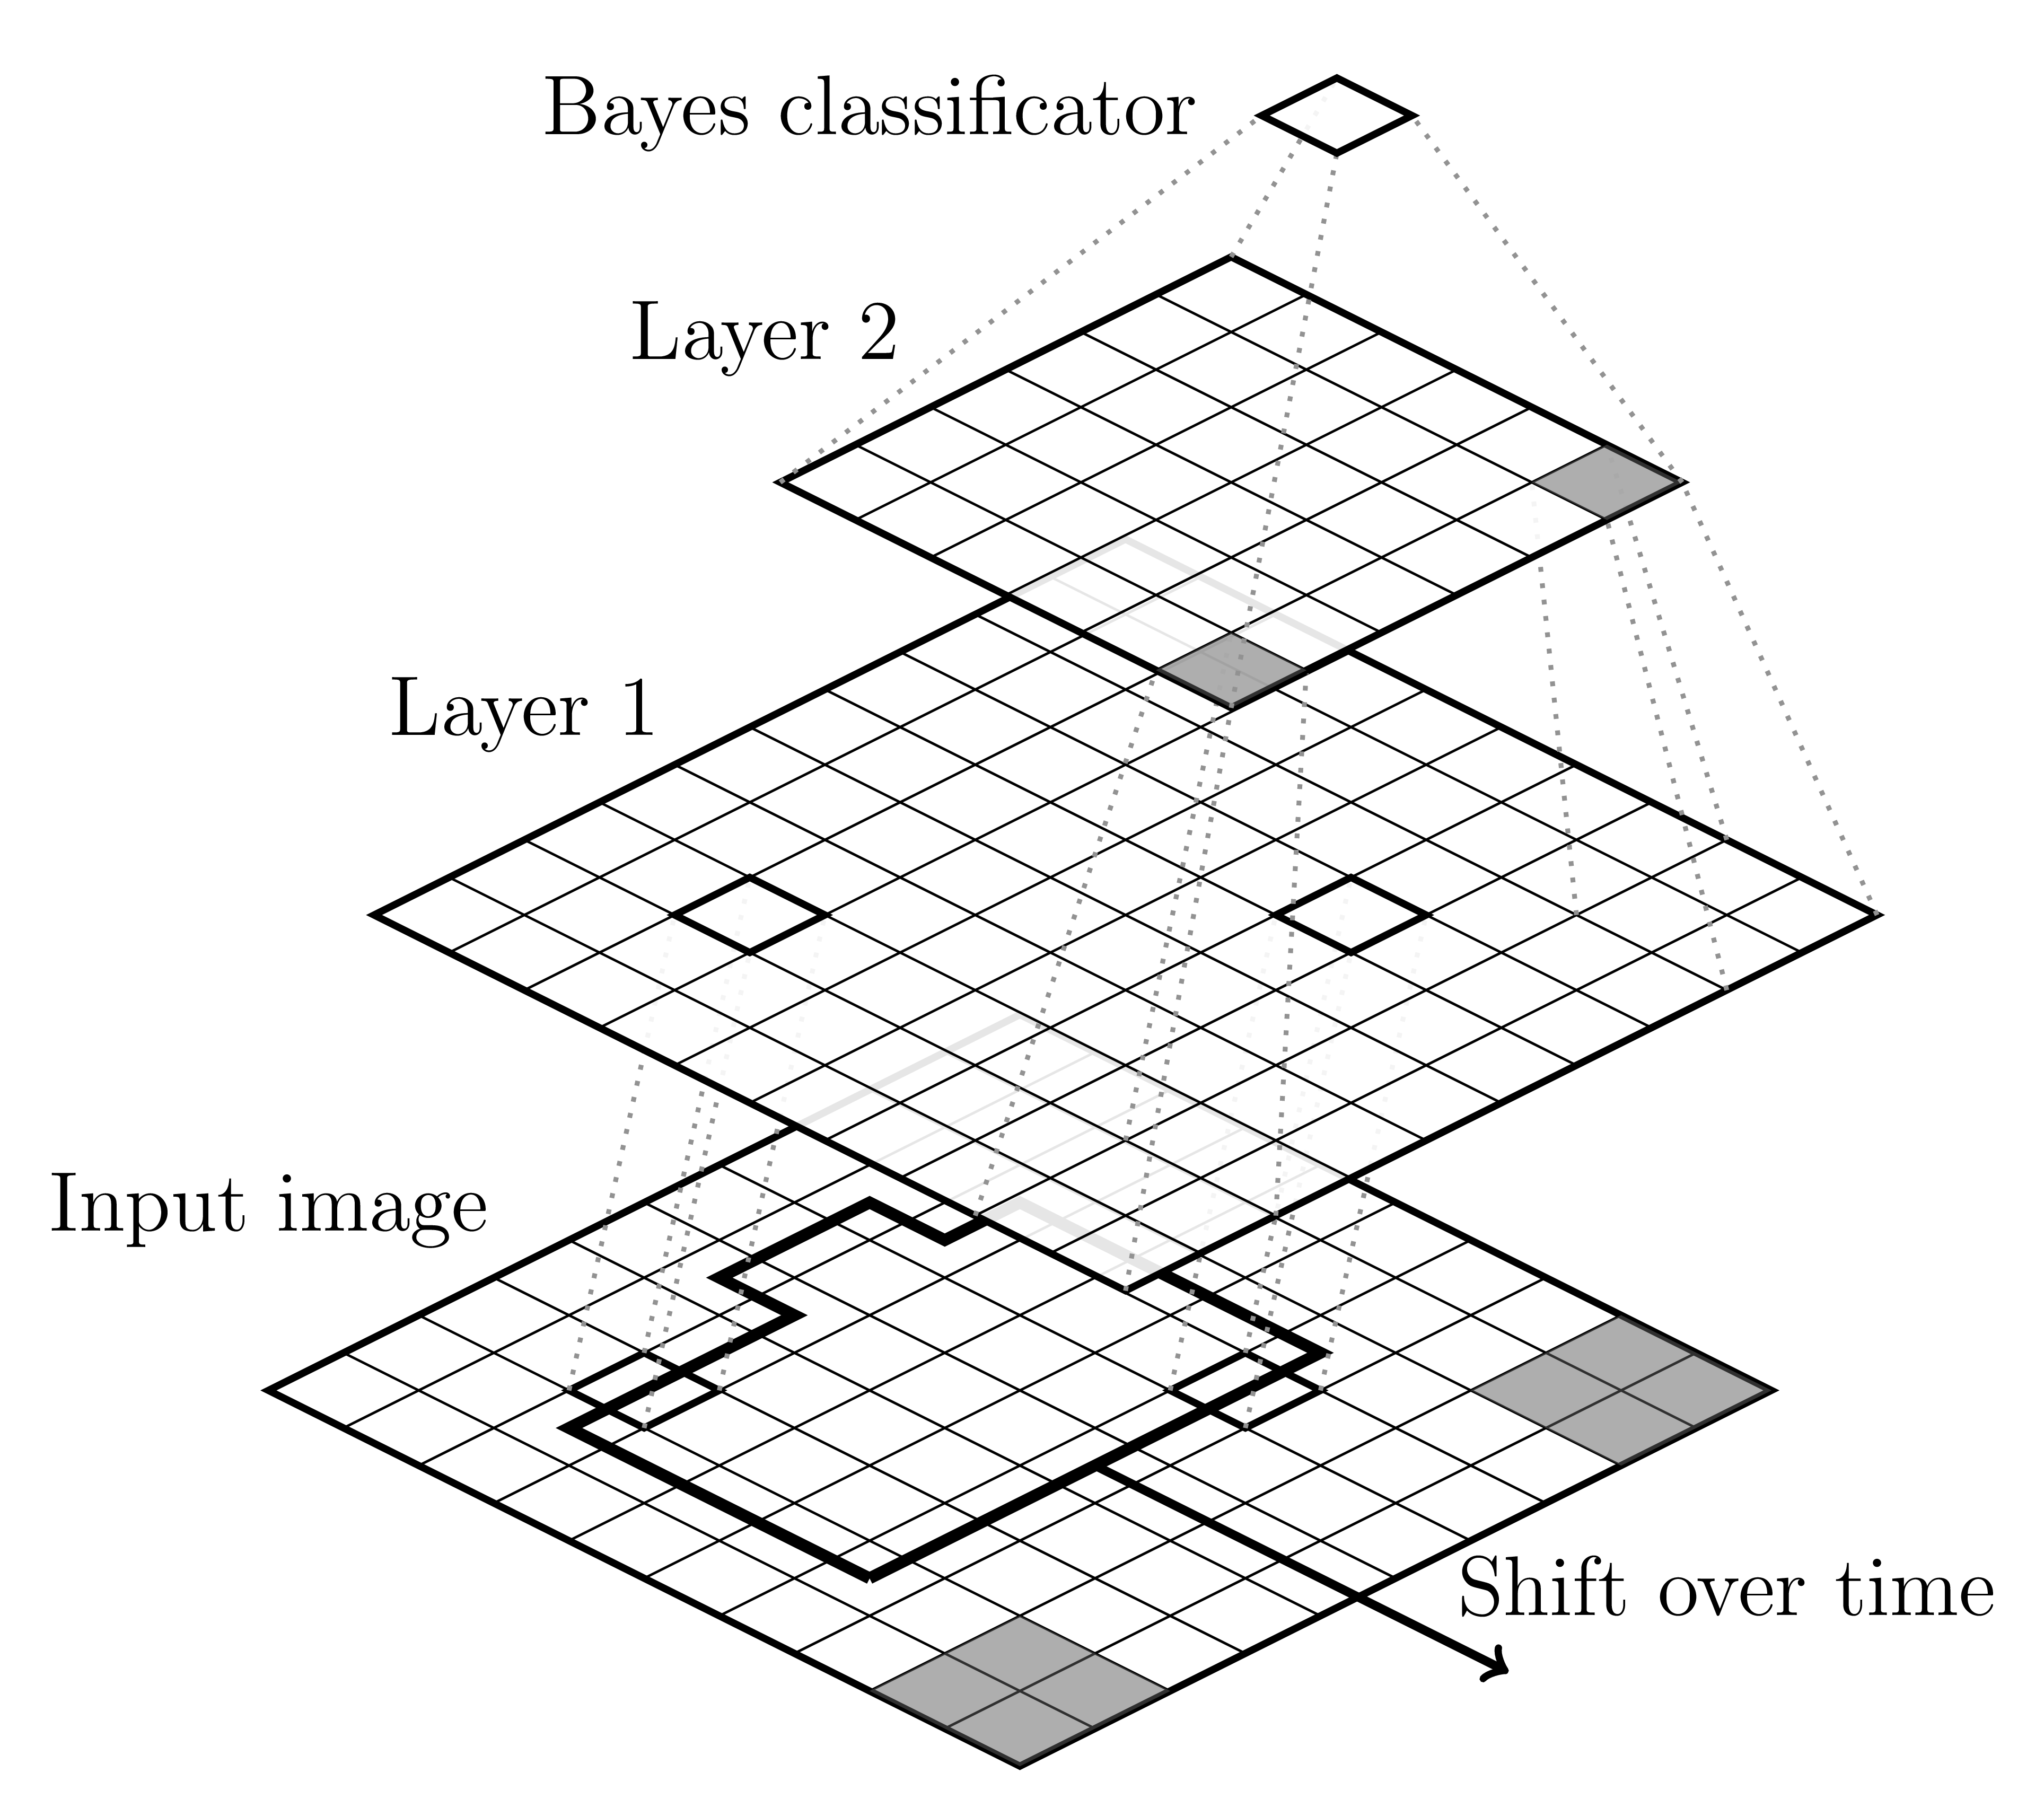
\includegraphics[width=0.7\textwidth]{rsm_toy_example2-0.png}
		};
		\node[draw, inner sep = 1pt, rectangle,thick] at (0,0) {
			
\includegraphics[width=.25\textwidth]{screen0.png}
		};
		\node[draw, inner sep = 1pt, rectangle,thick] at (3.2,0) {
			
\includegraphics[width=.25\textwidth]{screen1.png}
		};
		\node[draw, inner sep = 1pt, rectangle,thick] at (0,-3.2) {
			
\includegraphics[width=.25\textwidth]{screen2.png}
		};
		\node[draw, inner sep = 1pt, rectangle,thick] at (3.2,-3.2) {
			
\includegraphics[width=.25\textwidth]{screen3.png}
		};
		\node[inner sep = 1pt] at (12,-1.8) {
			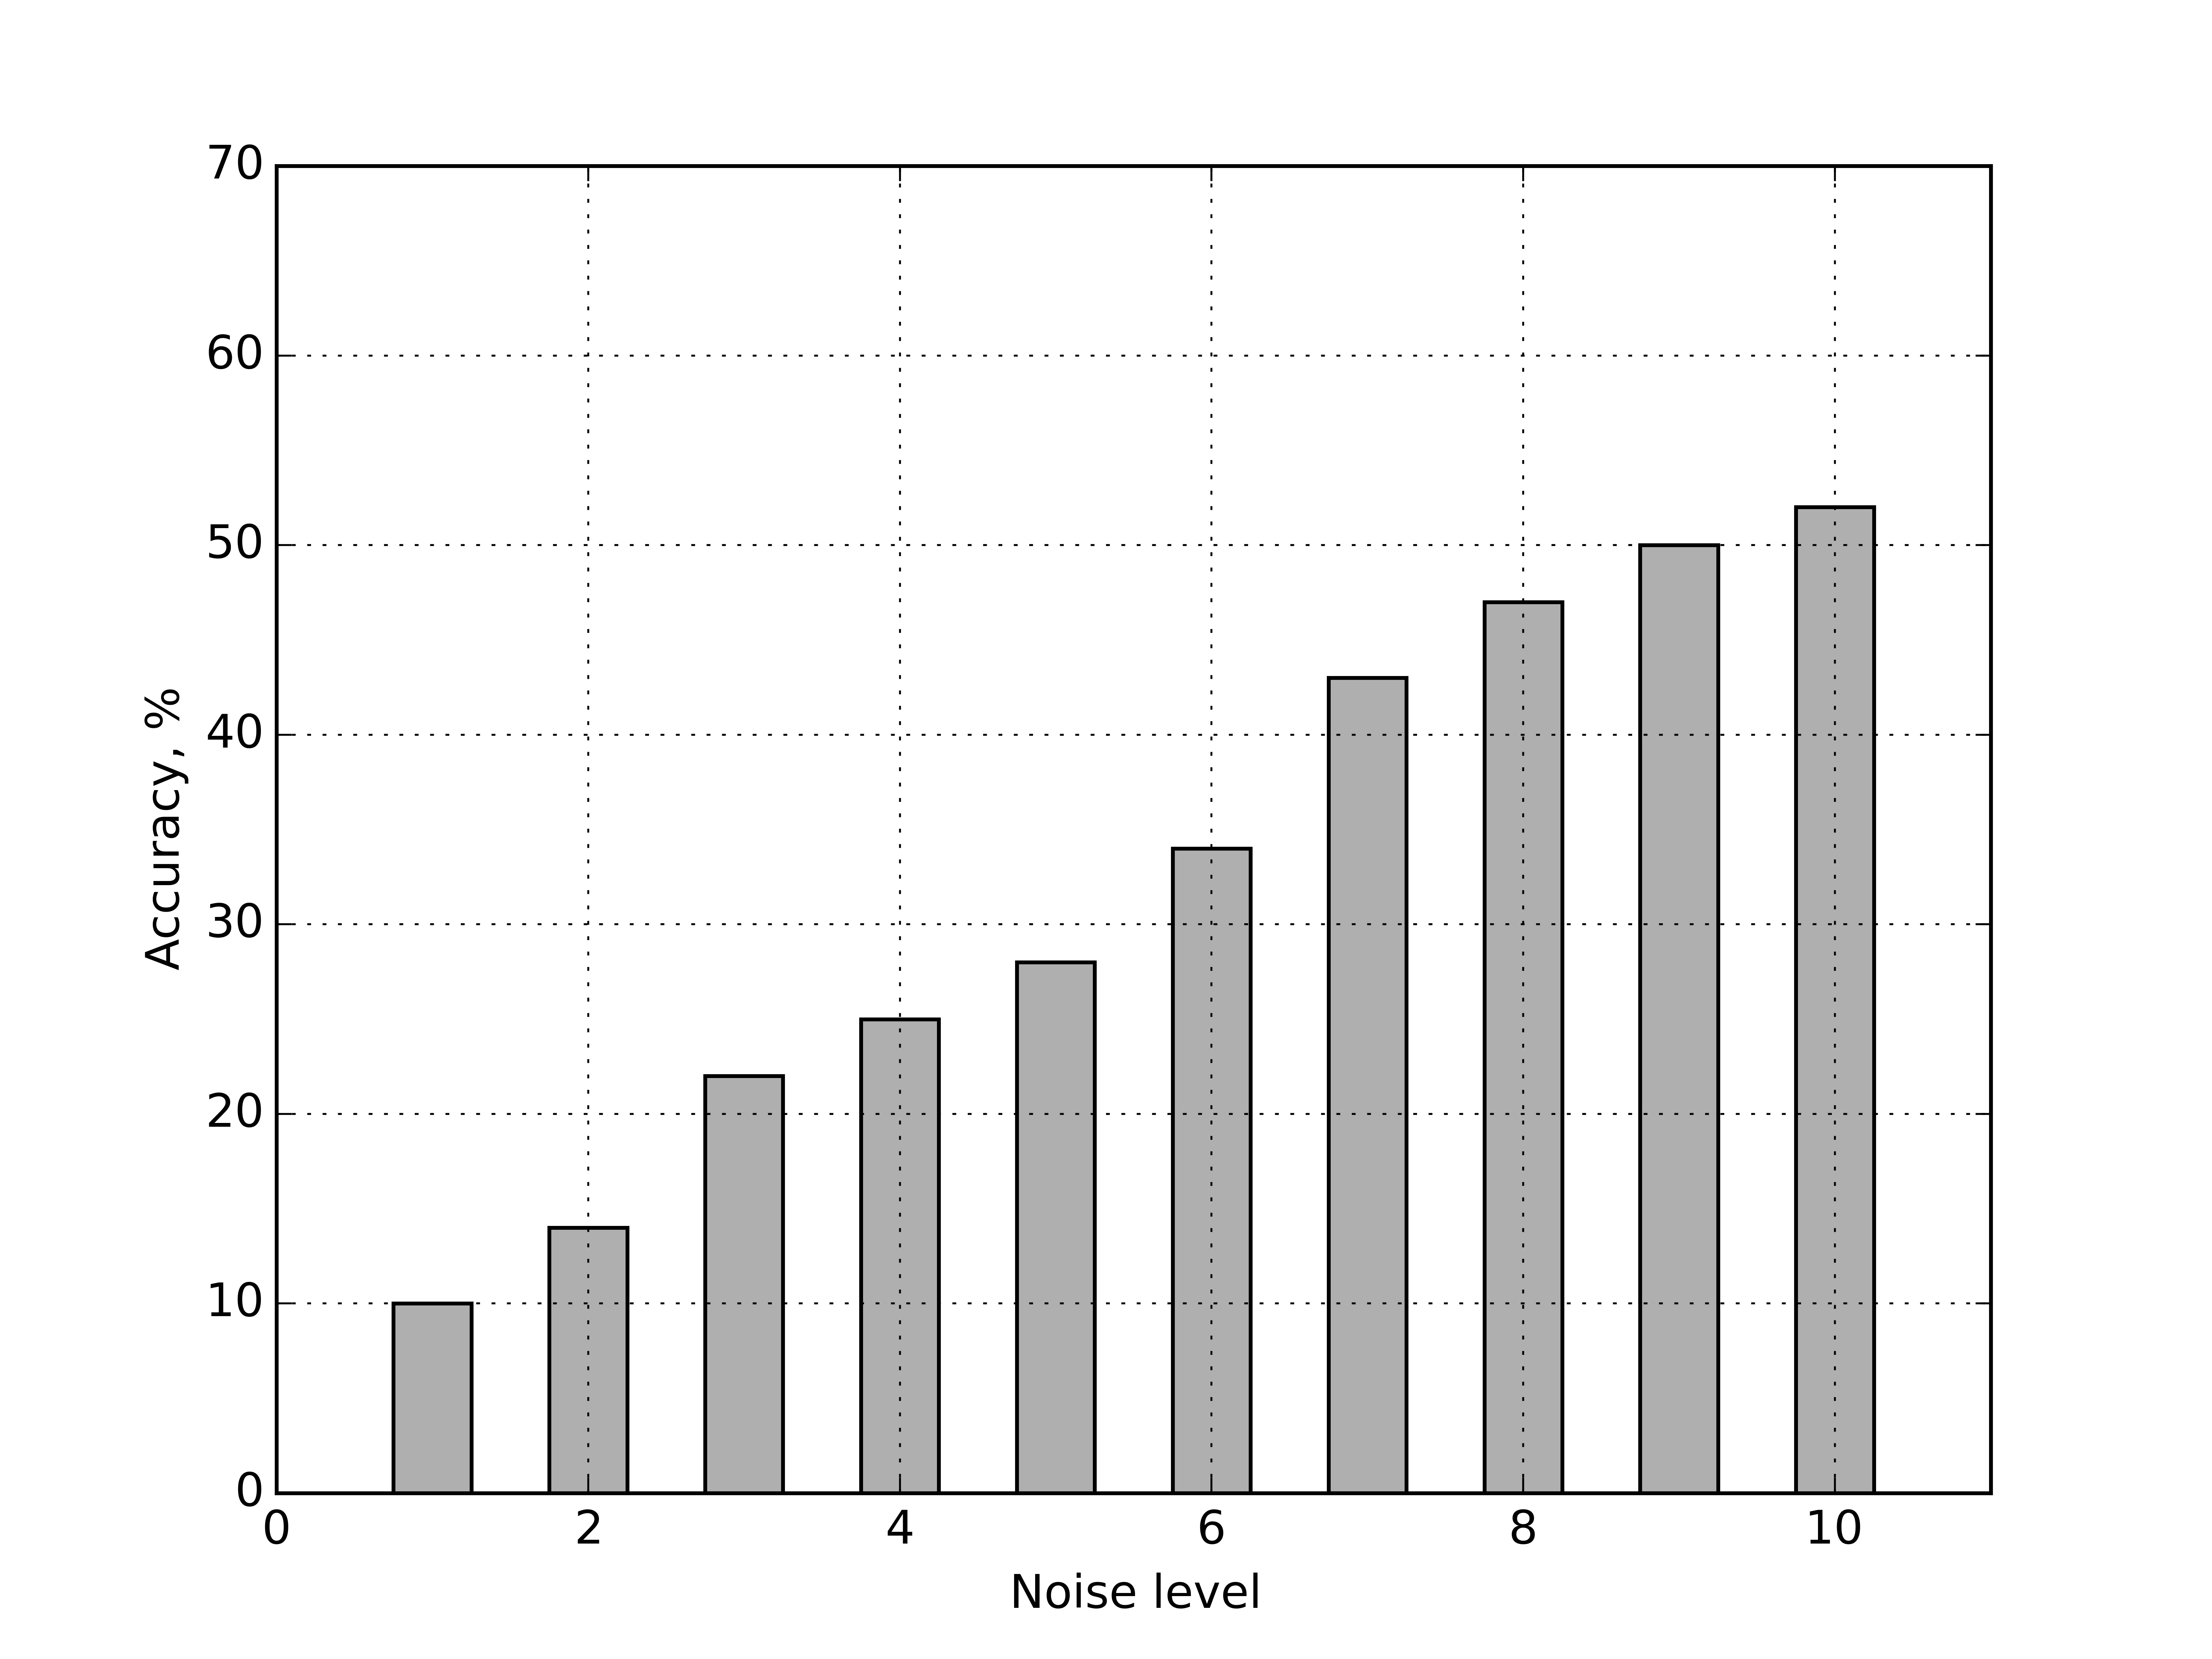
\includegraphics[width=\textwidth]{hist.png}
		};
		
		\node[font=\Large] at (-8, -7) {a)};
		\node[font=\Large] at (1.6, -7) {b)};
		\node[font=\Large] at (12, -7) {c)};
	\end{tikzpicture}
\end{document}